\providecommand{\main}{../../../..}
\documentclass[\main/dresen_thesis.tex]{subfiles}
\begin{document}
  \label{sec:doubleLayers:vsm}

  \begin{figure}[tb]
    \centering
    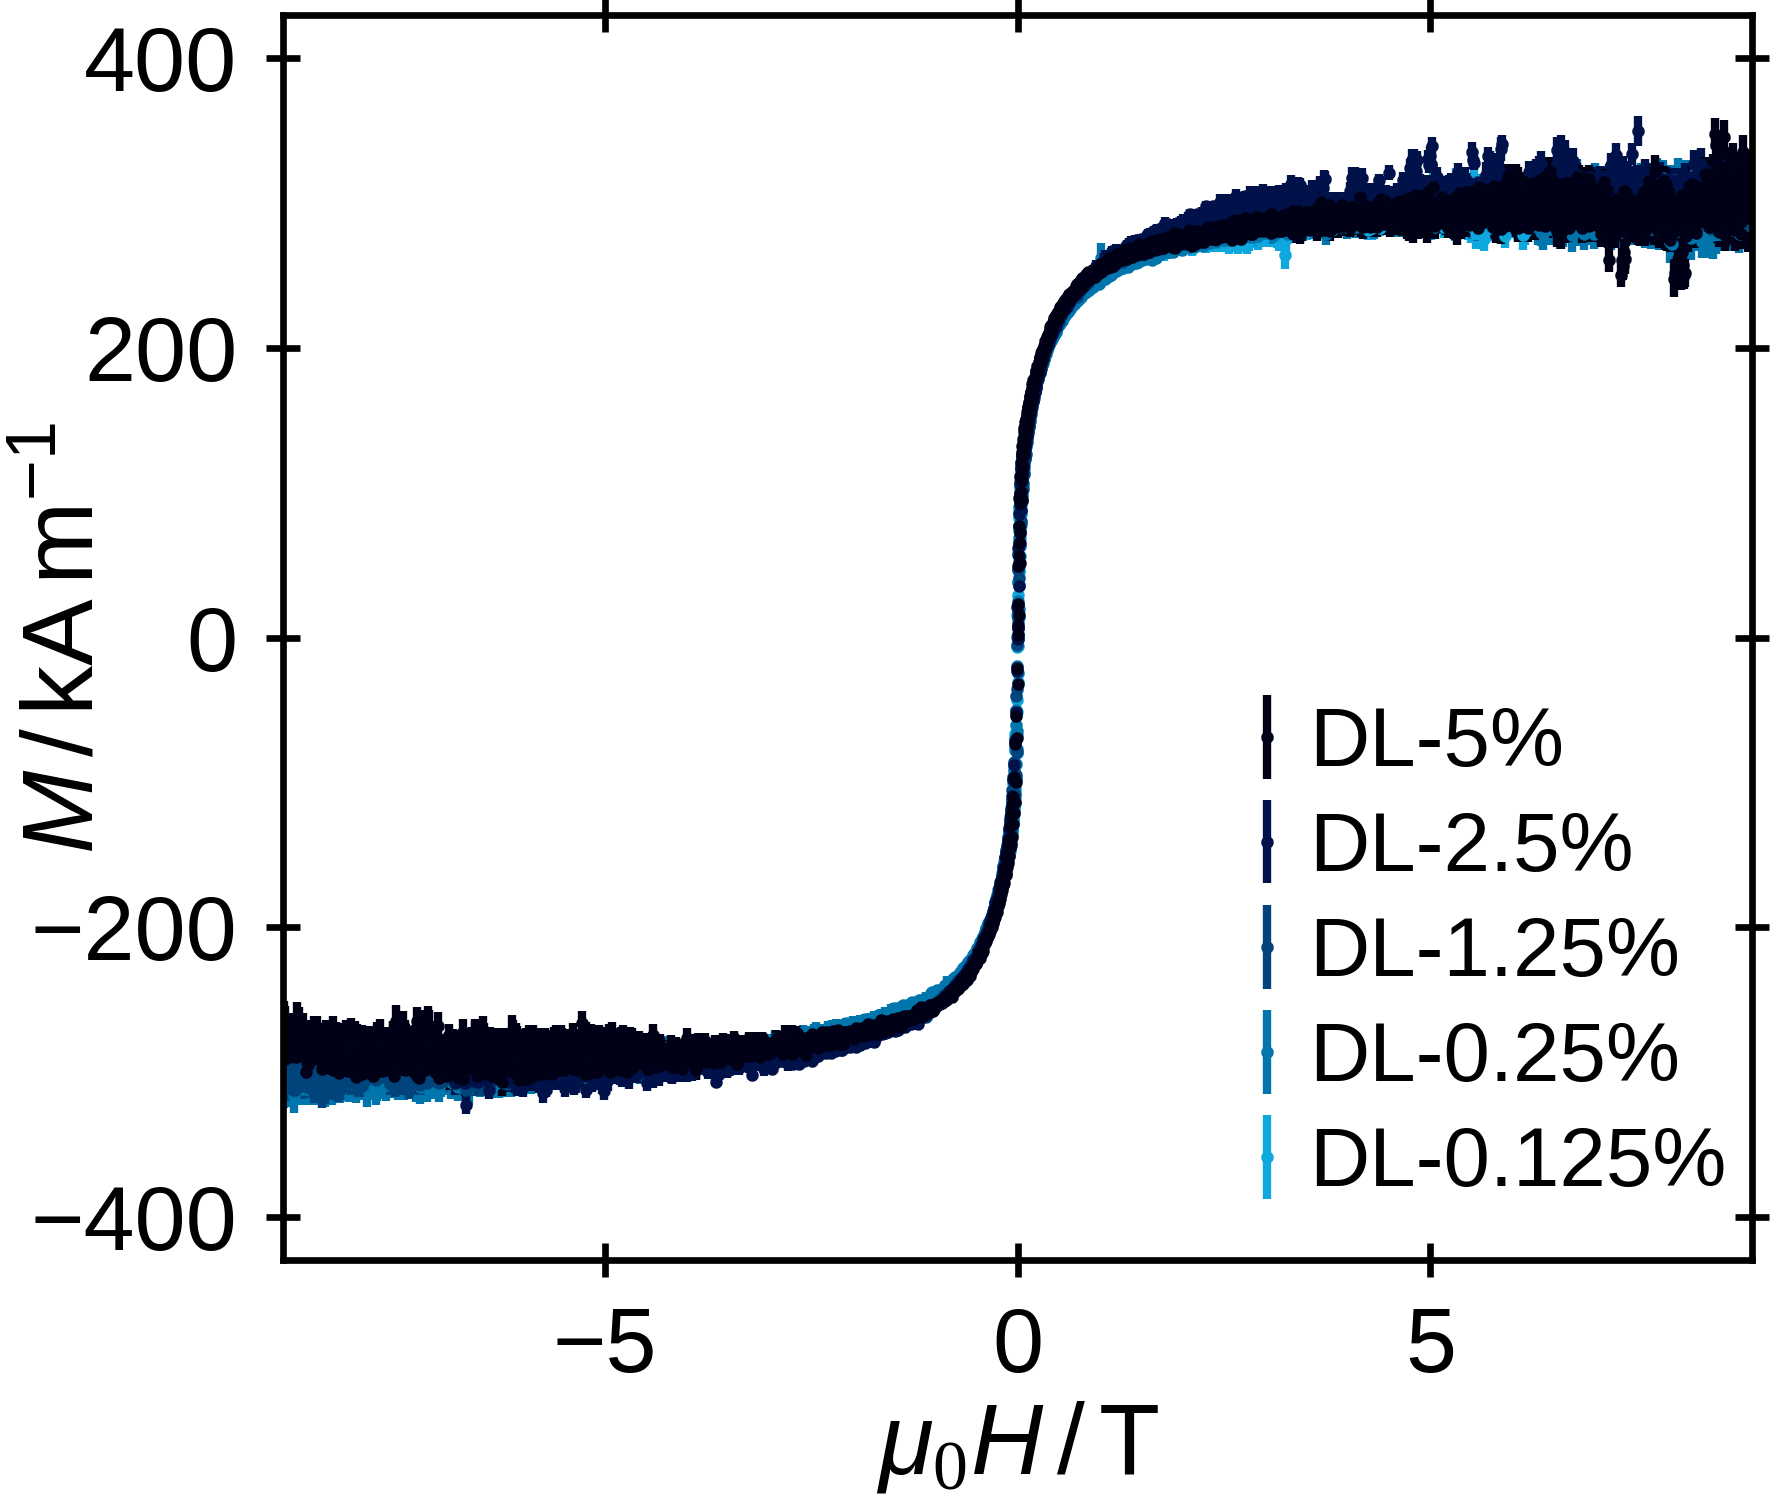
\includegraphics{doublelayers_PPMS_300K_allSamples}
    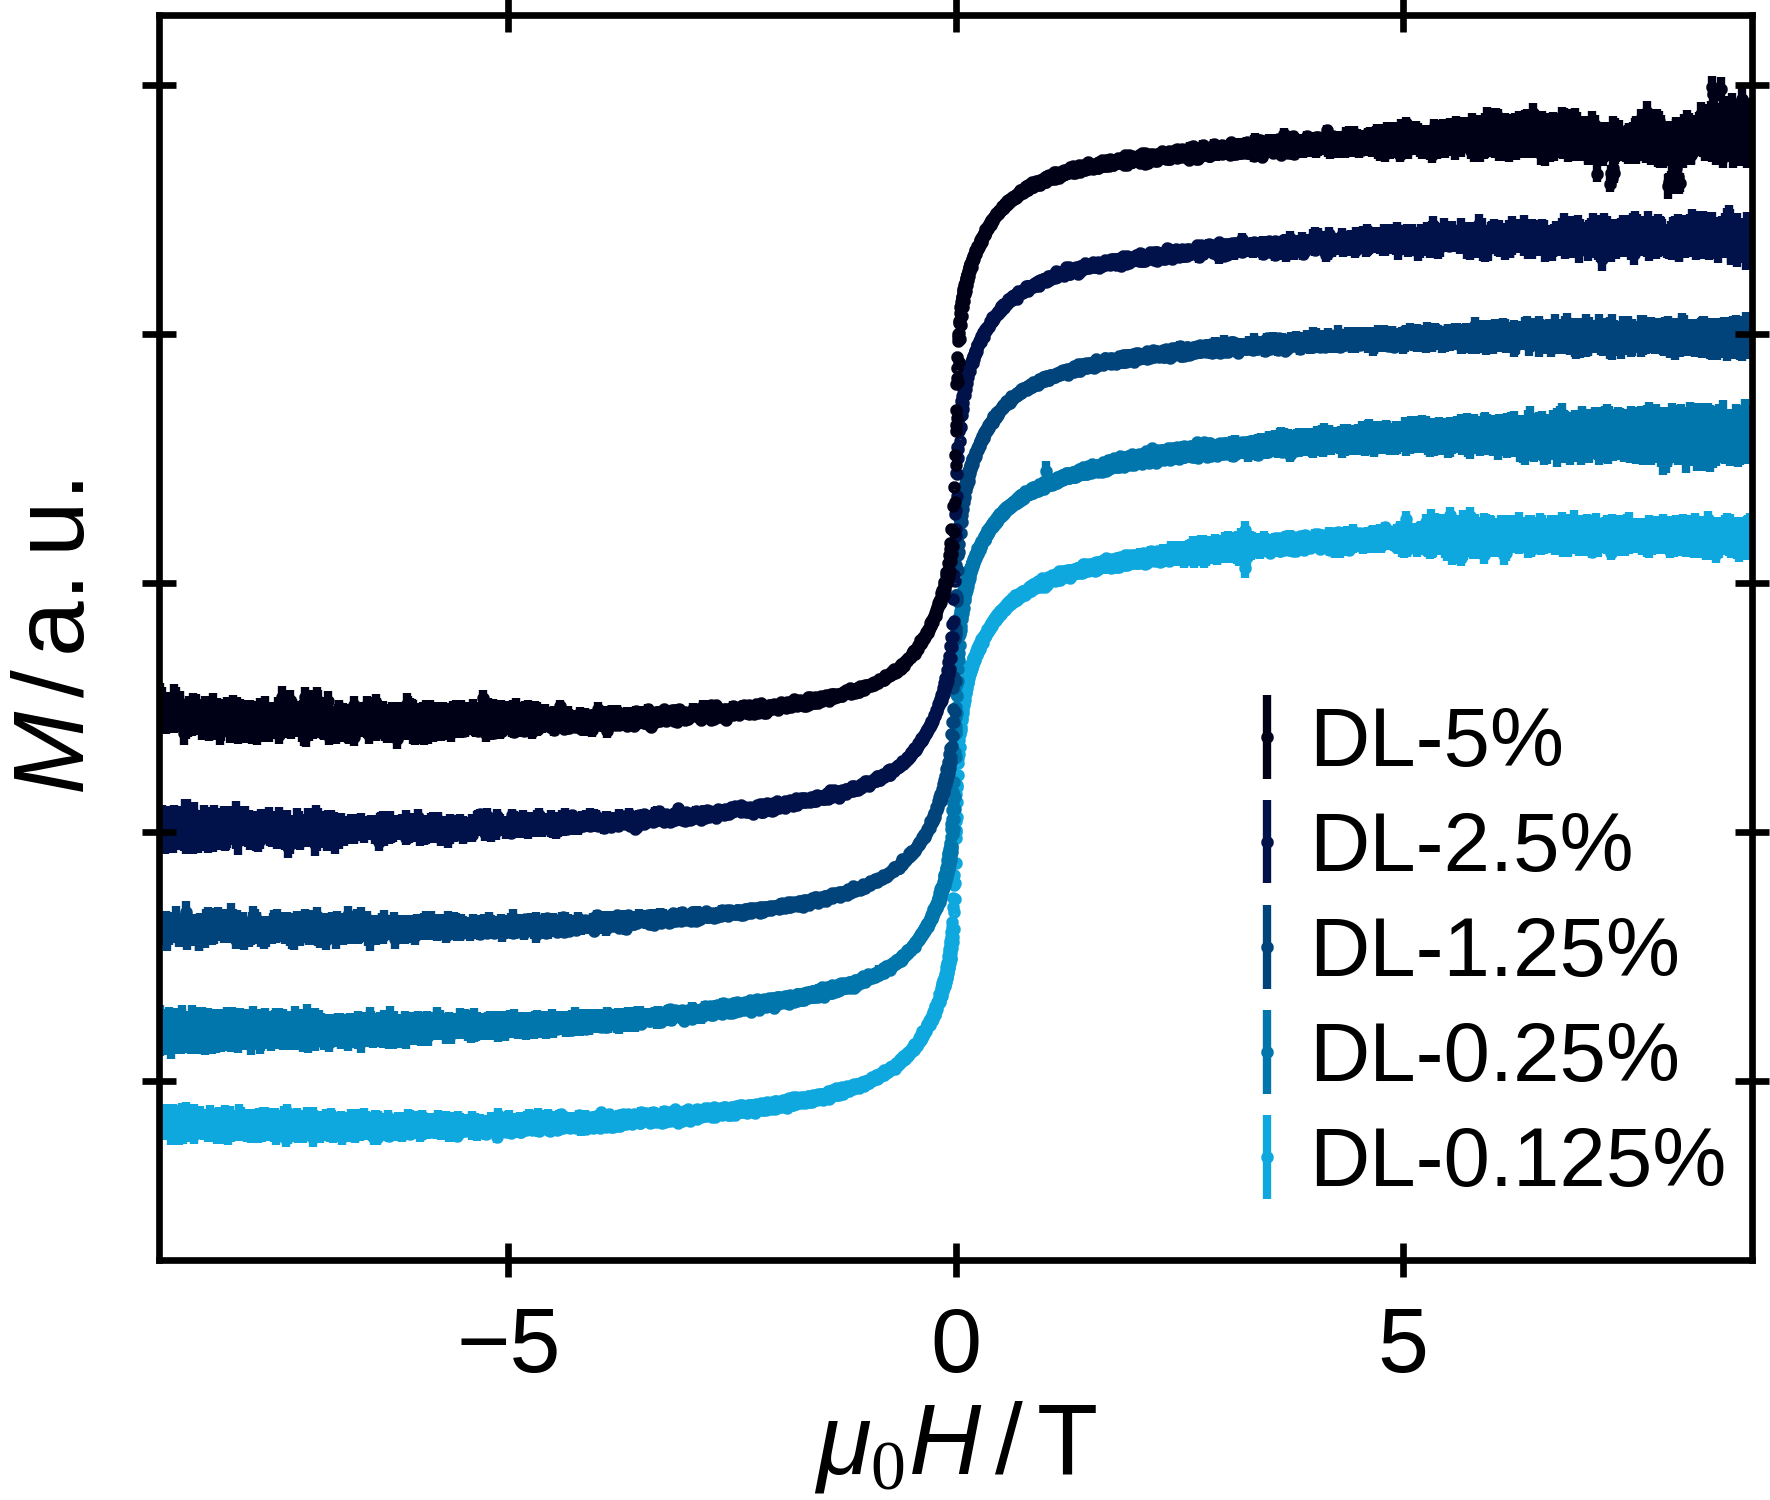
\includegraphics{doublelayers_PPMS_300K_allSamplesShifted}
    \caption{\label{fig:doubleLayers:RTVSM}Room temperature field-dependent magnetization of the double layer samples (left). The magnetizations are also shifted with respect to each other for direct comparison (right). The data is corrected for the diamagnetic susceptibility of the background and scaled to the observed spontaneous magnetization given in \reftab{tab:doubleLayers:RTVSM:parameters}.}
  \end{figure}

  \paragraphNewLine{Scaling of the Data and Silicon Background}
    Each double layer has been measured field- and temperature-dependent with the same procedure and conditions for direct comparison of the magnetic properties.
    As each double layer sample is prepared from the same dispersion and with a similar procedure, differences in the magnetic properties should be attributable to dipolar interlayer coupling as the PMMA thickness is the only varied parameter.
    Slight deviations are given in the sample size that is measured in the VSM due to the finite precision in breaking of the sample.
    In \reftab{tab:doubleLayers:RTVSM:parameters}, the determined susceptibility $\tilde{\chi}$ and spontaneous magnetization $\tilde{M}_s$ obtained from the room temperature measurements by a linear fit in the range of $5 - 9 \unit{T}$ is tabulated.
    As all  magnetic samples are assumed to be two layers of nanocubes and the susceptibility should be given by the size of the silicon substrate, the variation in the spontaneous magnetization and susceptibility should only be given by the variation of the sample size.
    Therefore, the values are also shown as scaled to the sample area, which accounts for the different cut sizes.

    \begin{table}[!htbp]
      \centering
      \caption{\label{tab:doubleLayers:RTVSM:parameters} Spontaneous magnetization and susceptibility of the double layer samples determined by fitting the slope of the field-dependent room temperature magnetization in the range of $5 - 9 \unit{T}$.}
      \begin{tabular}{ l | l | l || l | l}
        \rule{0pt}{2ex} \textbf{VSM}  & $M_s \, / \unit{\musf emu}$ & $\chi \, / \unit{\musf emu \, T ^{-1}}$ & $\bar{M}_s \, / \unit{\musf emu \, mm^{-2}}$ & $\bar{\chi} \, / \unit{\musf emu \, T^{-1} mm^{-2}}$ \\
        \hline
        \rule{0pt}{2ex} DL-0.125\%   & $87.2(2)$   & $-36.96(3)$ & $3.56(1)$ & $-1.509(1)$\\
        \rule{0pt}{2ex} DL-0.25\%    & $83.6(3)$   & $-35.58(4)$ & $3.68(1)$ & $-1.565(1)$\\
        \rule{0pt}{2ex} DL-1.25\%    & $87.4(2)$   & $-33.78(3)$ & $3.94(1)$ & $-1.525(1)$\\
        \rule{0pt}{2ex} DL-2.5\%     & $88.5(5)$   & $-36.02(7)$ & $3.62(2)$ & $-1.566(2)$\\
        \rule{0pt}{2ex} DL-5\%       & $90.2(5)$   & $-39.78(8)$ & $3.59(2)$ & $-1.585(4)$\\
        \hline
      \end{tabular}
    \end{table}

    For the rescaled values, the mean susceptibility is $-1.55\, / \unit{\musf emu \, T ^{-1} mm^{-2}}$ with a relative standard deviation of $2.0 \%$  and the mean spontaneous magnetization is $3.7 \, / \unit{\musf emu \, mm^{-2}}$ with a relative standard deviation of $4.2 \%$.
    The susceptibility can be compared to the literature value for an equivalent pure silicon layer of $0.52 \unit{mm}$ thickness, which is $-1.34\, / \unit{\musf emu \, T ^{-1} mm^{-2}}$ \cite{Lide_2004_Handb}.
    The higher experimental value and fluctuations of the susceptibility after scaling to the silicon mass accounts for the varnish that is used to fix the sample, which is of varying amount.
    For the spontaneous magnetization the fluctuations after scaling to the silicon mass tells that slight variations are given in the nanocube content in each double layer.
    This is connected to the finite precision of the pipettes that are used to transfer the nanocubes from dispersion to the substrate during drop casting.

    As no strong interaction effects are expected at room temperature, the samples are scaled using the measured spontaneous magnetization, such that relative changes after cooling to low temperatures can become more visible.
    The diamagnetic contributions are also subtracted from the data, as they are arguably a pure signal from the silicon substrate.
    The spontaneous magnetization is then set analogue to the treatment of the monolayer sample in \refsec{sec:monolayers:magneticStructure:vsm} to the value expected from the single particle magnetic moment from the nanocubes in dispersion measurement and the particle size determined by SAS.
    The resulting room temperature magnetizations that closely resemble each other after correction are shown in \reffig{fig:doubleLayers:RTVSM}.
    The data is shown once plot on top of each other to show the close match and once with a constant shift for better differentiation of the respective datasets.
    The determined scaling factors by the spontaneous magnetization and the same diamagnetic correction are applied to the low temperature field-dependent and temperature-dependent measurements without further modification.


  \paragraphNewLine{Temperature-dependent magnetization}

    \begin{figure}[tb]
      \centering
      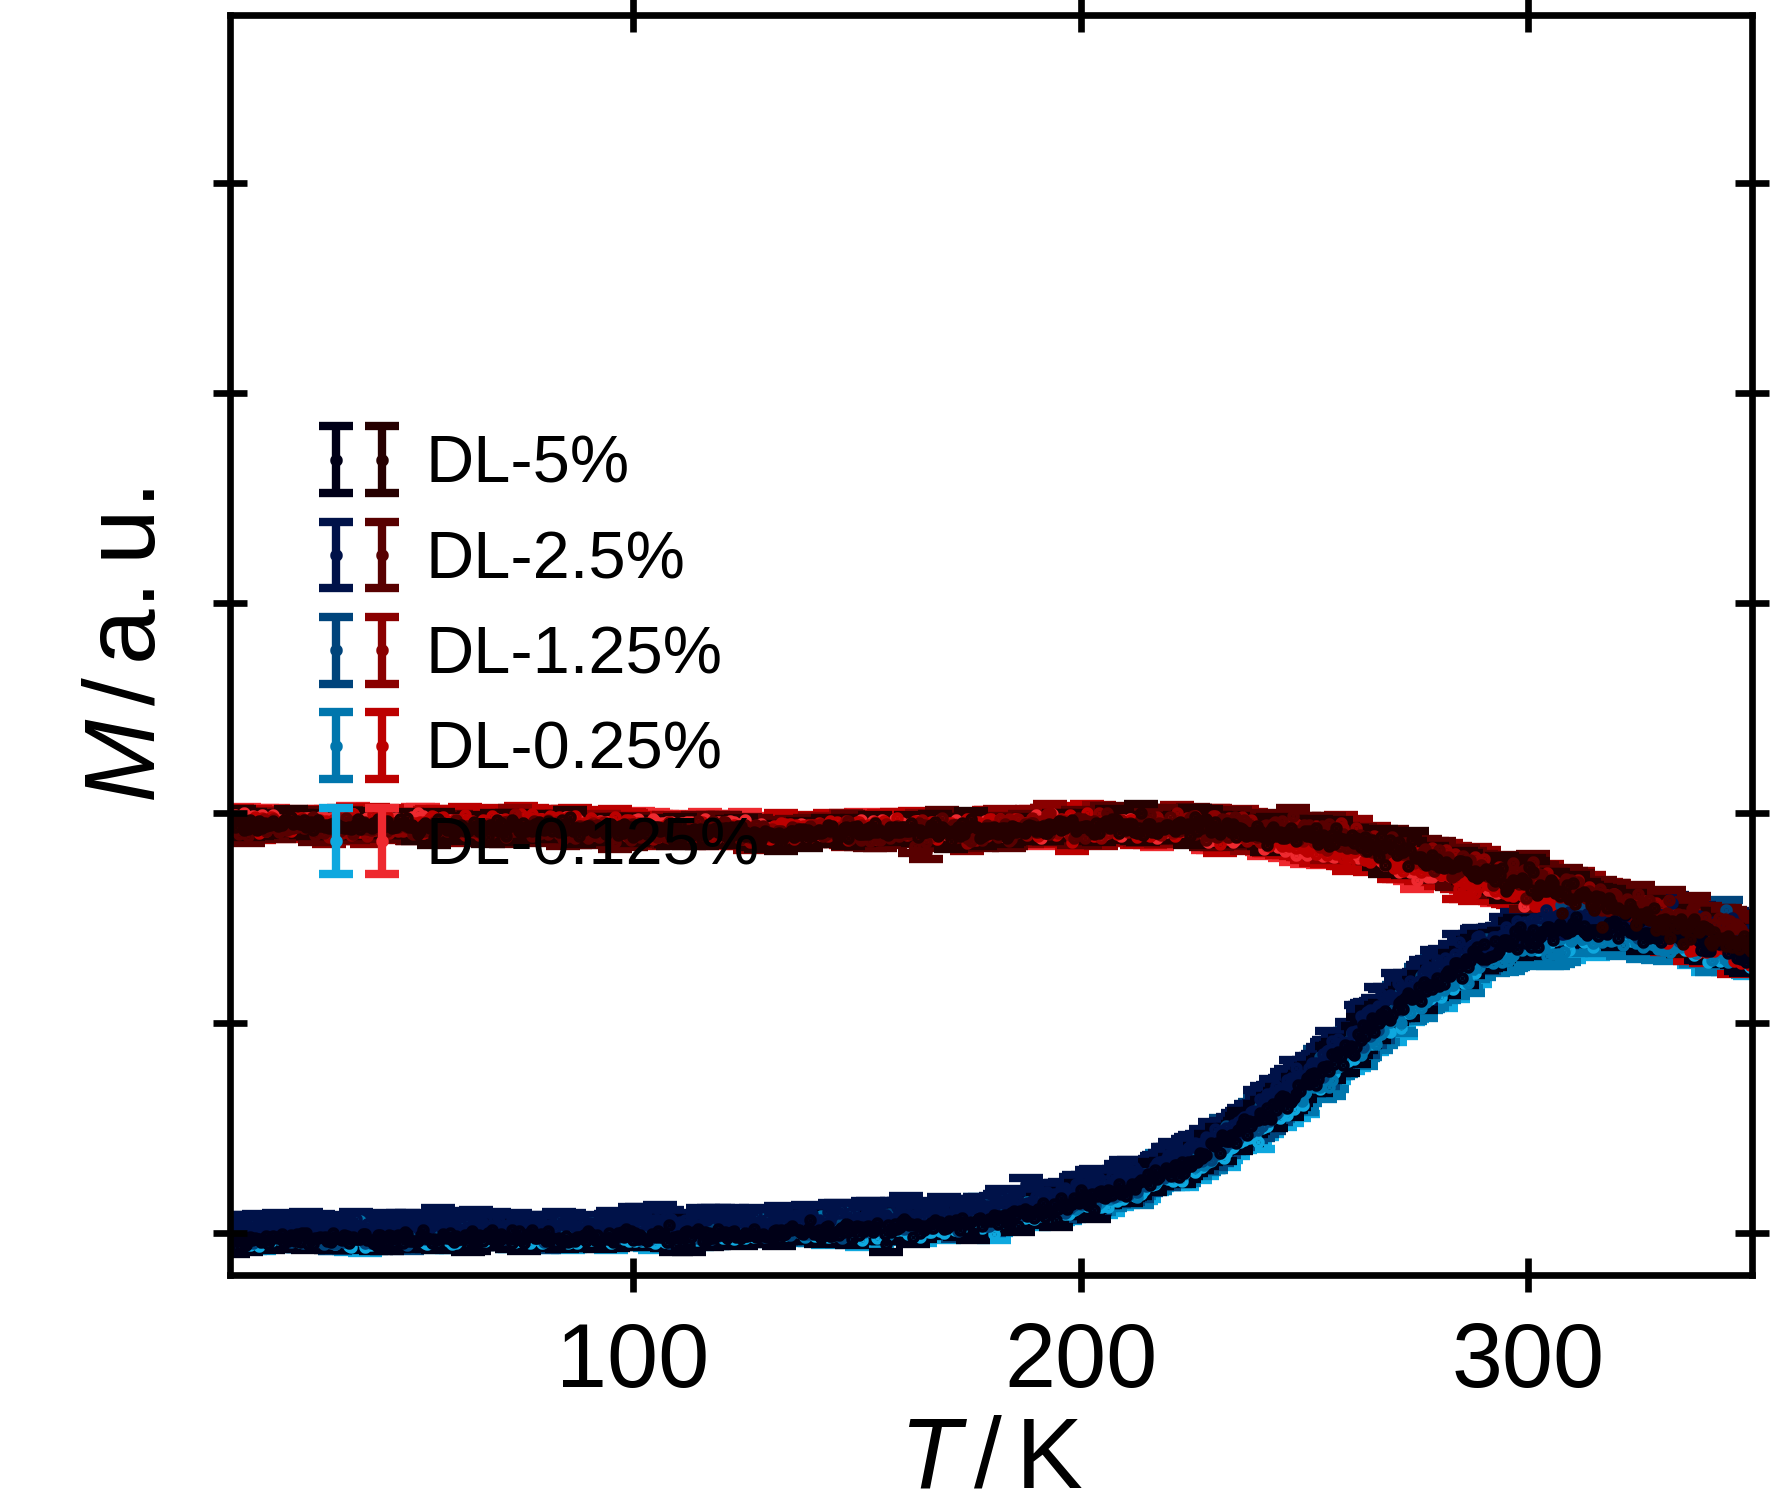
\includegraphics{doublelayers_PPMS_ZFC_FC_allSamples}
      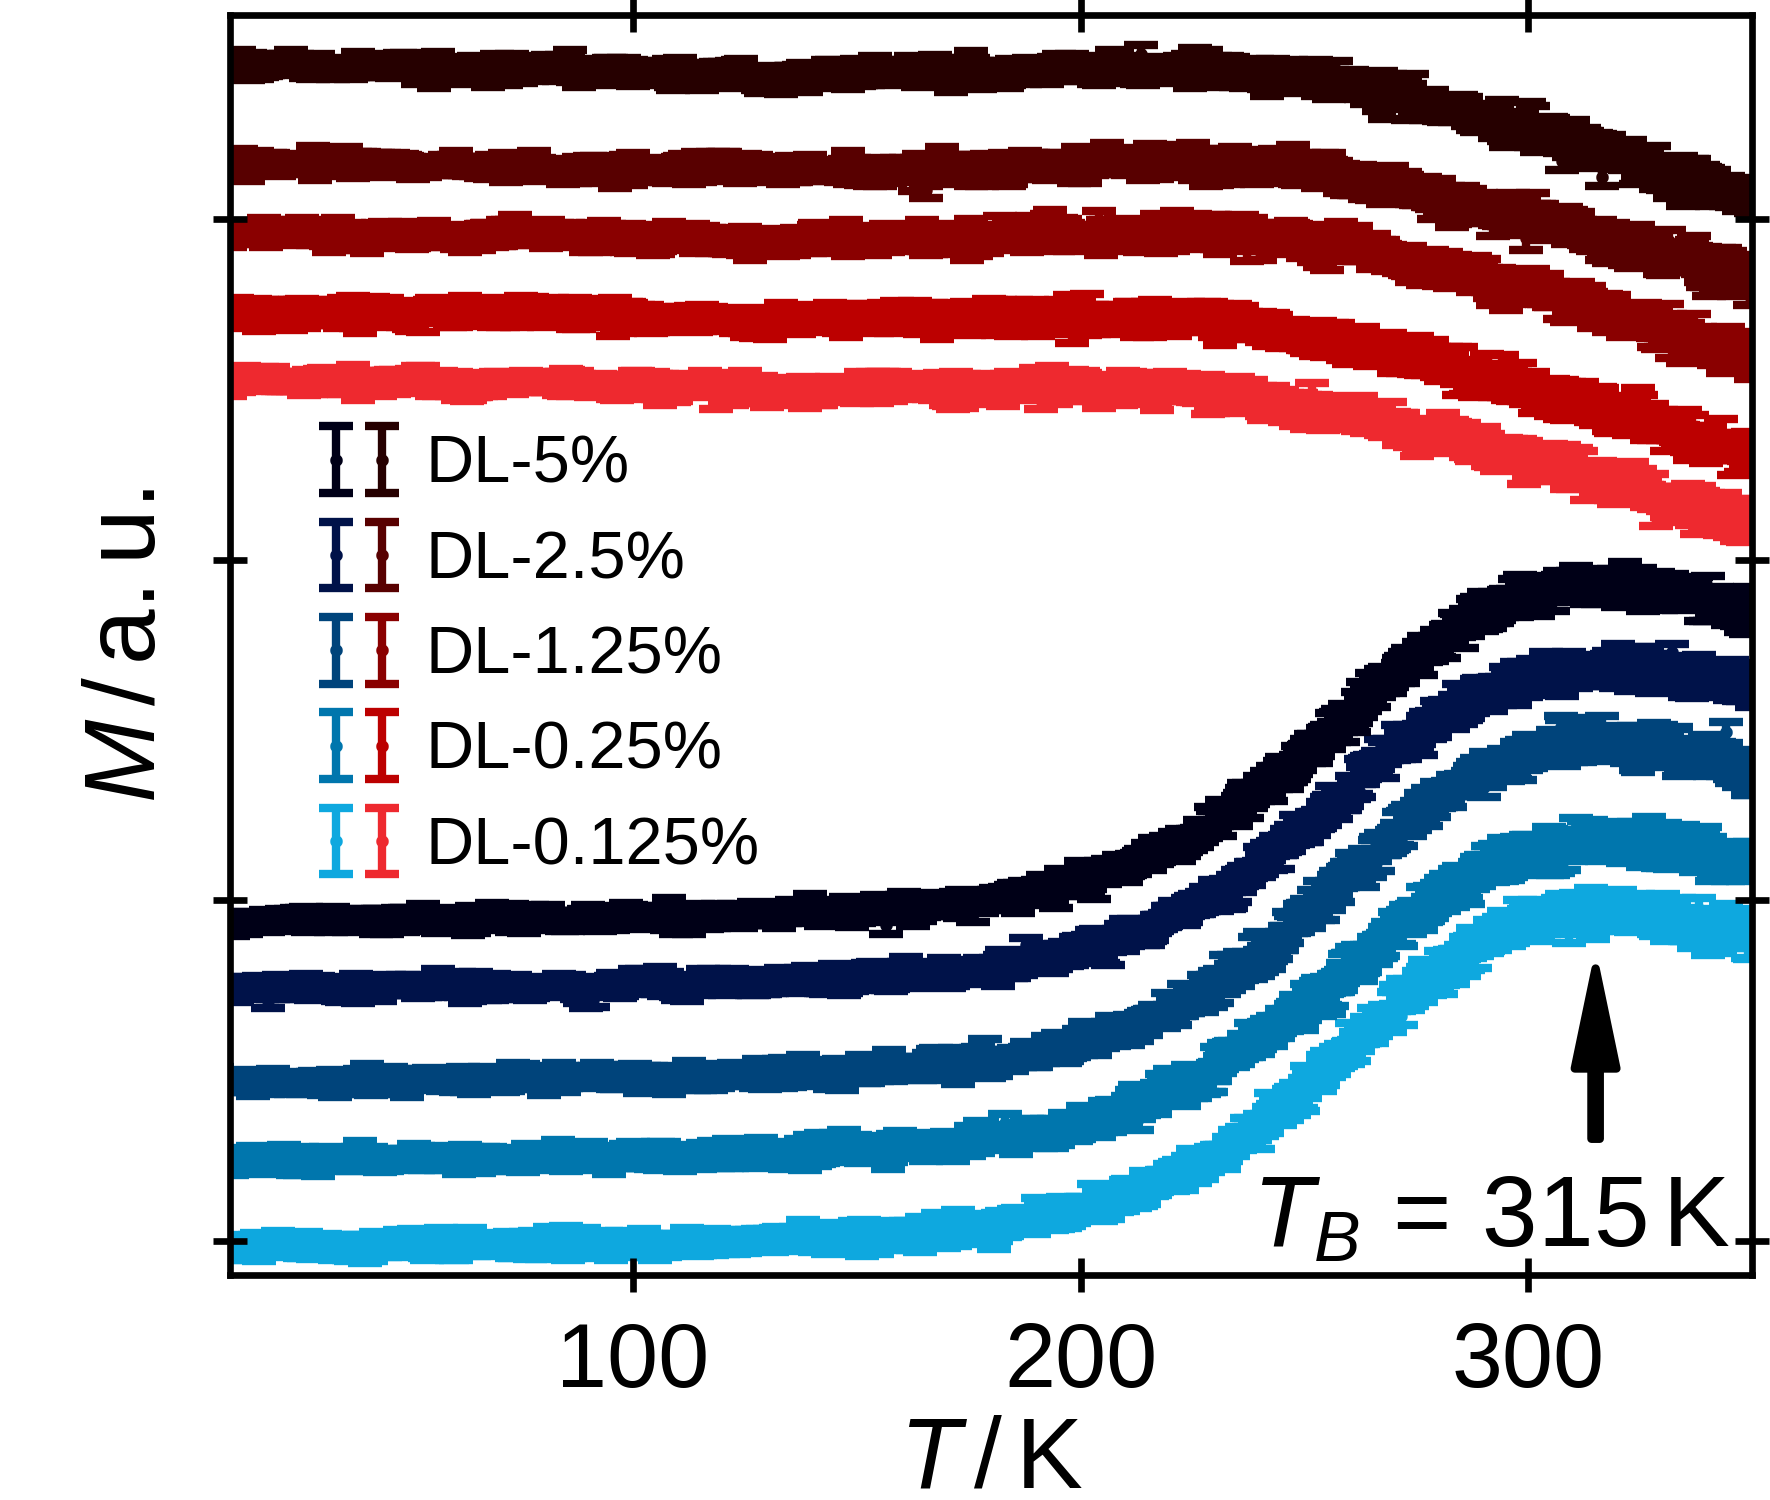
\includegraphics{doublelayers_PPMS_ZFC_FC_allSamplesShifted}
      \caption{\label{fig:doubleLayers:zfcFCData}Temperature-dependent magnetization of the double layers (left). The ZFC/FC magnetizations are taken with a field of $10 \unit{mT}$ while warming the sample. To discuss the qualitative differences, the zero-field cooled and field cooled data, as well as the respective data of the samples with varied spacer thicknesses are shifted by a constant factor (right).}
    \end{figure}
    In \reffig{fig:doubleLayers:zfcFCData} the temperature-dependent magnetization is shown for the double layer samples, sorted with respect to the varied PMMA thickness.
    A close inspection of temperature dependent magnetization shows that they all closely resemble each other and no significant difference can be observed across the samples.
    A small difference can be seen in the initial magnetization measured after zero-field and field cooling, which is however close within the error margins and has no strong correlation to the sample thickness.
    Similar to the monolayer sample in \refsec{sec:monolayers:magneticStructure:vsm}, a blocking temperature around $315 \unit{K}$ is observed as peak temperature in the zero-field cooled magnetization.
    No major shift in that peak position can be observed within the resolution of the measurement, which could otherwise have been a sign for interlayer interaction.
    It can therefore be concluded that if interlayer interaction has an effect on the double layer magnetization, it is below the resolution of the temperature-dependent measurement.

  \paragraphNewLine{Field-dependent low temperature magnetization}

    \begin{figure}[tb]
      \centering
      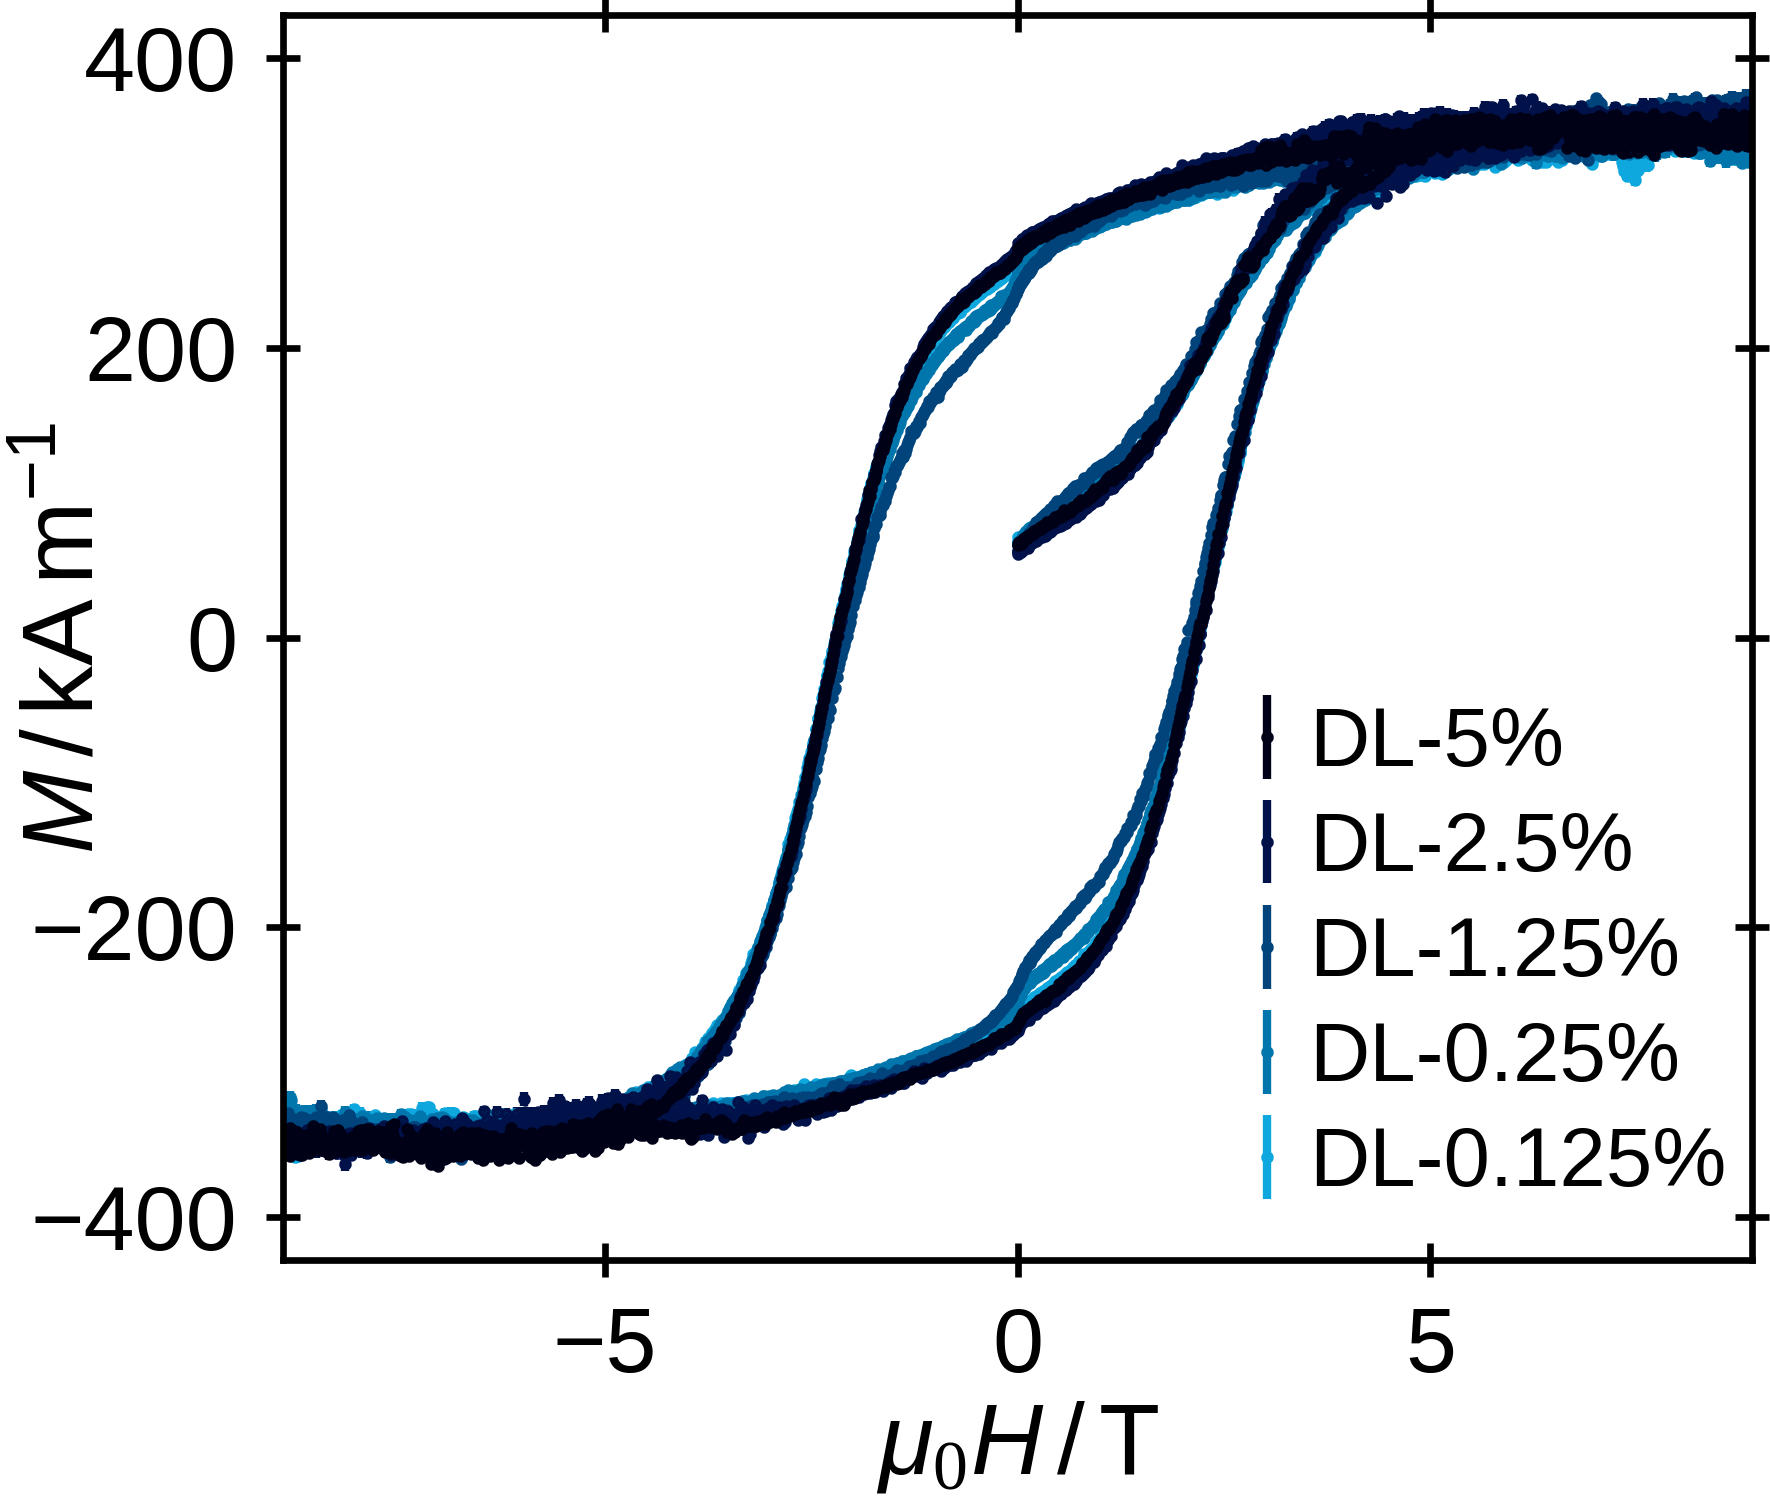
\includegraphics{doublelayers_PPMS_10K_allSamples}
      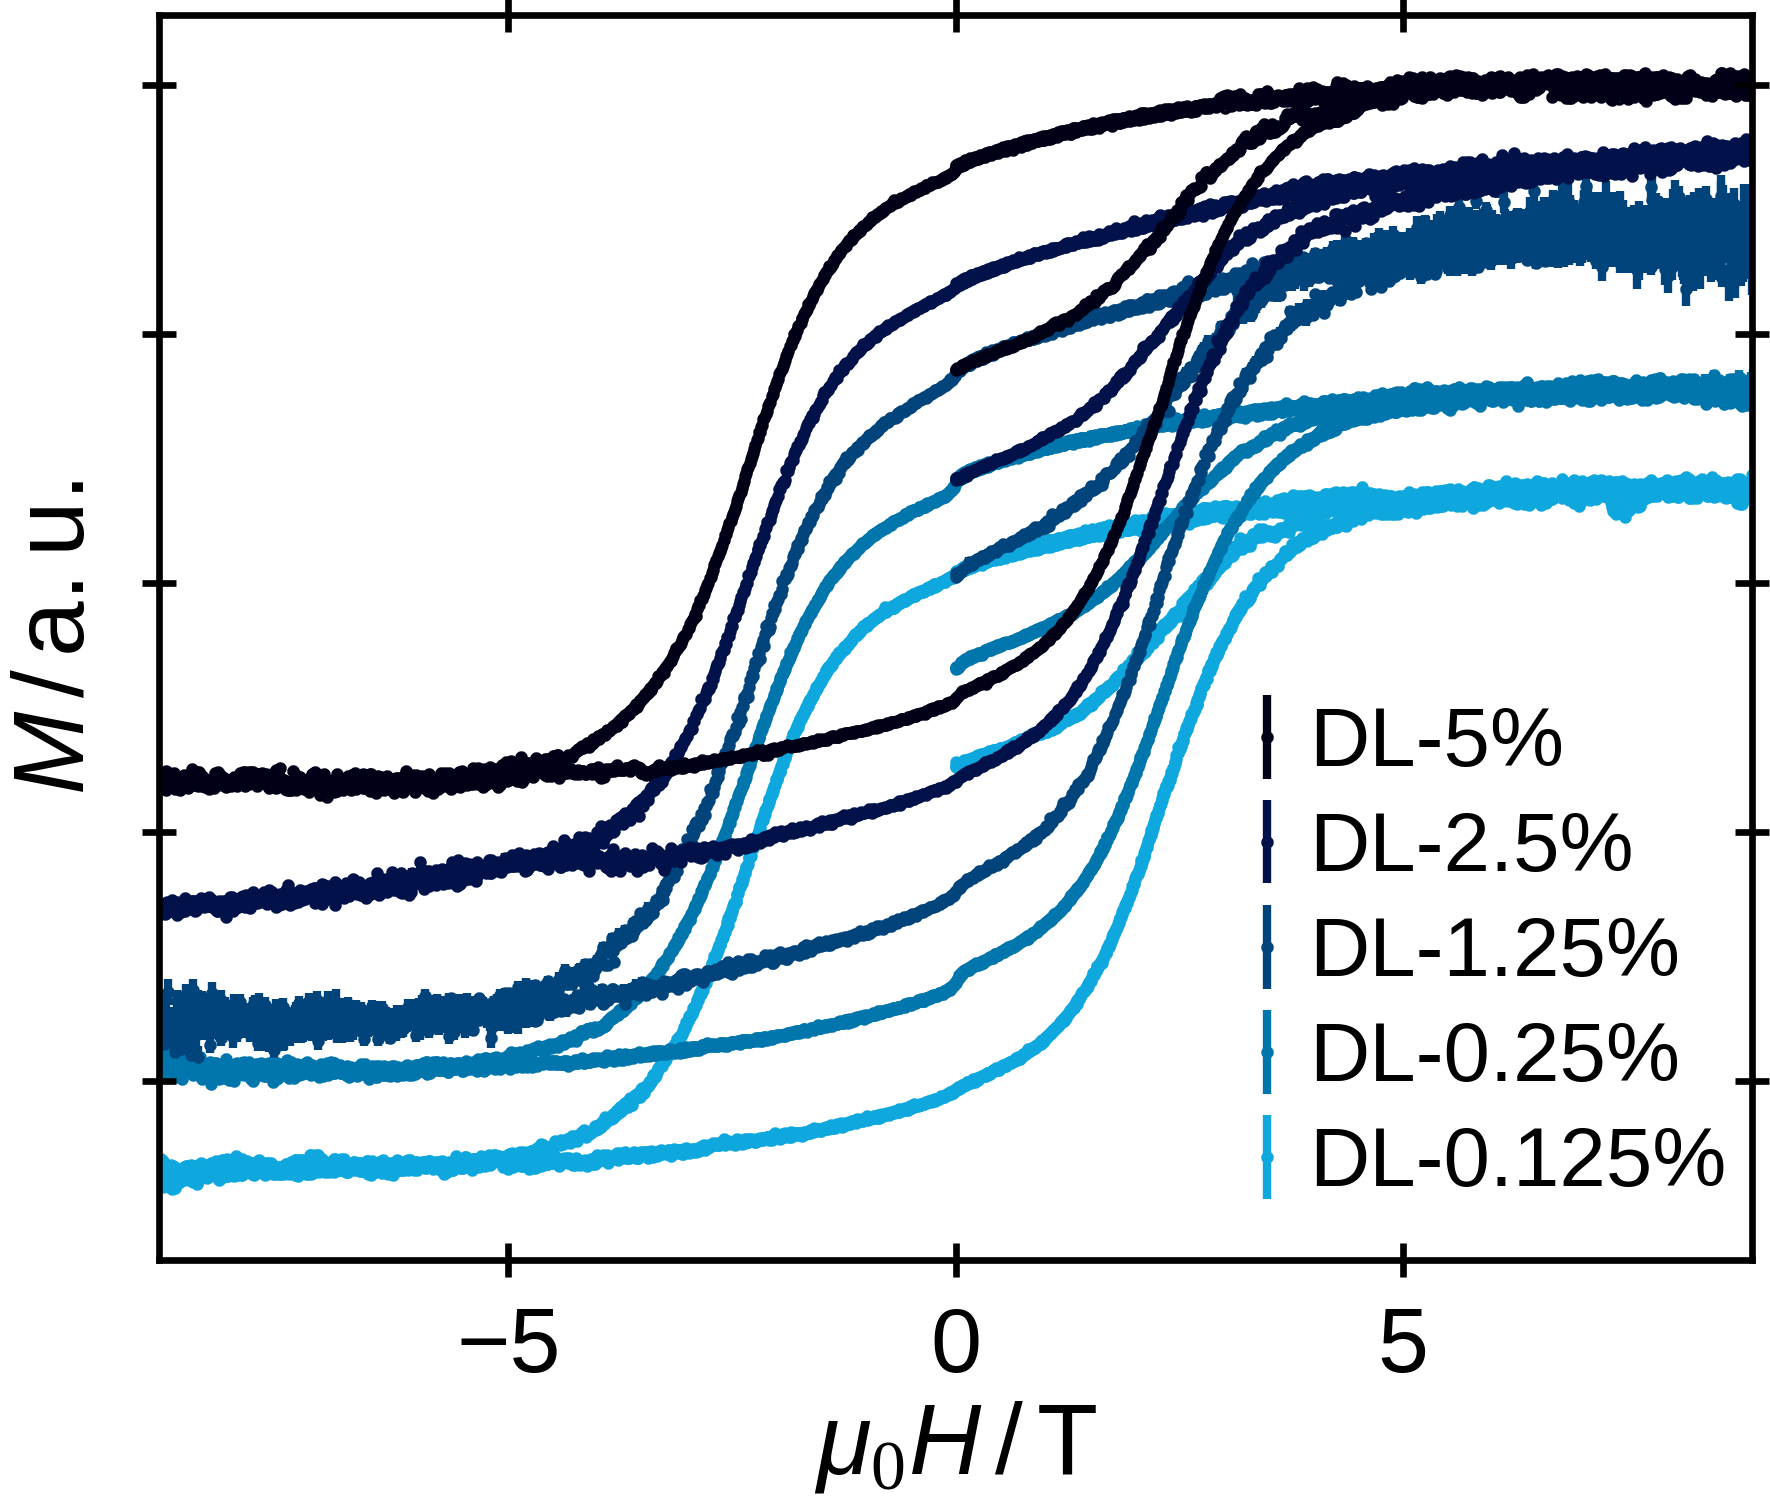
\includegraphics{doublelayers_PPMS_10K_allSamplesShifted}
      \caption{\label{fig:doubleLayers:10KVSM}Field-dependent magnetization of the double layers measured at $10 \unit{K}$ after cooling in a $10 \unit{mT}$ field (left). Similar to \reffig{fig:doubleLayers:RTVSM} the hysteresis curves are shifted by the same factor for differentiation (right). Additionally the virgin curves are masked for clarity.}
    \end{figure}
    Stronger variations can be seen in the hysteresis at $10 \unit{K}$.
    Similar to the monolayer sample in \refsec{sec:monolayers:magneticStructure:vsm}, a small jump in the magnetization is visible around $\pm 100 \unit{mT}$ in all samples.
    The magnitude of the jump is visibly changing from sample to sample, without showing a direct systematic with respect to the PMMA layer thickness but is directly correlated to the magnitude of the spontaneous magnetization measured for the samples at room temperature in \reftab{tab:doubleLayers:RTVSM:parameters}.
    Whereas it is very small for the lowest PMMA concentration sample DL-0.125\%, it appears clearly visible for DL-0.25\%, and even larger for DL-1.25\% before it reduces again for DL-2.5\%, DL-5\%.
    Not observing a strong jump in DL-0.125\% and an increase in DL-1.25\% in comparison to DL-0.25\% is out of the expectation when the origin of this jump is considered to be due to an antiferromagnetic coupling between the two layers, as this is expected to monotonously reduce in strengh with increasing interlayer distance.
    Furthermore, as the jump also appears in monolayer samples, it is probable that this effect is not directly correlated to interlayer interaction but a property of the single nanocube arrays themselves.
    As discussed in the section about the magnetic properties of the non-interacting nanoparticles \refsec{sec:monolayers:nanoparticle:vsm} and the monolayer section in \refsec{sec:monolayers:magneticStructure:vsm}, this jump is observed by multiple sources in literature, where some sources suggest that the nature of the jump is due to surface spin effects of the nanocubes \cite{Xu_2015_Simul, Fu_2012_Uniqu}, and others show a connection to dipolar interparticle interaction \cite{Alves_2017_Waspw, Sathya_2016_Cofeo}.
    The direct comparison of the magnetic behaviour of the nanoparticles frozen in a dispersion, in a sample without long-range order and within a long-range ordered monolayer in \reffig{fig:monolayer:magneticStructure:MLAcCoFeCCompareDispWafer}, indicated that for the studied nanocubes dipolar interparticle interactions are the most probable origin for the jump.
    And it was furthermore observed that with long-range order in the monolayer the jump actually reduces in magnitude, which is attributed to a super ferromagnetic coupling in the monolayer.

    In the coercive field, the hysteresis curves of all samples up to DL-1.25\% resemble each other closely with a  magnitude of $2.16(3) \unit{T}$, which is in agreement with the monolayer sample.
    For DL-1.25\% a smaller coercive field of $2.06(1) \unit{T}$ is observed.
    Comparing this to the magnetization behaviour studied in the monolayer chapter, DL-1.25\% shows a tendency that is closer to the disordered monolayer with the higher jump and the smaller coercive field.
  \\

  Concludingly, the macroscopic magnetization characterization of the samples shows comparable magnetic properties across the double layer samples, with variations that are not directly correlated to the interlayer distance.
  To get a better understanding of the magnetic structure and to see if the interlayer interaction effects are possibly hidden in the magnetization data, polarized neutron reflectometry experiments have been proposed.

    % , where the sample shifted on the glass holder.

  % In literature, the jump can be found in multiple works discussing cobalt ferrite nanoparticles .
  % The authors give multiple explainations ranging from dipolar interaction between the particles, to surface spin reorientation, o
  % At the state of this thesis it is yet unclear what the true nature of the jump at low fields is.
\end{document}